%!TEX root = ../main.tex

%
% Notes: 
%
%  exact implementation
%  comparison with rollback at batch N
%  relaxing the solvers
%  dealing with false positives
%
%  running on TPC-C/sanjay's.  equality is easier
%
% Need names for
%  * rollback
%  * exact solution
%  * fixing an individual/batch of queries
%
\section{Experiments}

In this paper, we have described an exact, albeit less-scalable,
constraint-based solution to the \prob problem, as well as several
extensions to the solution that 1) trade off scalability with
diagnosis quality, and 2) support noise in the input complaint set.
Our goals in the evaluation is to understand these trade-offs in
controlled synthetic scenarios, as well as study the effectiveness
in typical database query workloads.

To this end, our experiments are organized as follows: First, we
study \exact on a small controlled, synthetic workload with a single
corrupted query and explore the parameters that make the problem
challenging.  Second, we decompose \exact into rollback and \qfix algorithms and study each
in isolation using a series of micro-experiments, as well as together in an end-to-end-system.  
Third, we add noise to the input complaint sets to evaluate \density, and study
number of corrupted queries to understand how our algorithms scale to 
based.  Lastly, evaluate on real-world workloads based on TPC-C as
well as a data-cleaning application.




%
% NOTE: figures are named <experimentsection>_<subsection>_<xaxis>.pdf
%

\subsection{Experimental Setup}

We ran a combination of synthetically generated query logs, and
well as logs generated using a subset of the TPC-C~\cite{tpcc}
transaction log that consists of inserts and updates.  In each
experiment, we corrupt the query log as described below, execute
the original and corrupt logs on an initial (possibly empty) database,
and compare the resulting database states to generate a true complaint
set.  We then add noise to the complaint set by adding false positive
complaints, and removing true complaints to simulate false negatives.
Finally, we execute \sys on the complaints and compare the fixed
query log with the true query log, as well as the fixed and true
final database states to measure performance and accuracy metrics.

\subsubsection{Metrics}

\begin{itemize}
\item {\it Fixrate}: Percentage of true complaints correctly modified
\item {\it Err}: Percentage of errors introduced
\item {\it $Cost_{all,preproc,prep,solver}$}: Execution times overall ($cost_{all}$), 
      pre-processing time for XXX ($cost_{preproc}$), time for constructing the problem that is
      passed to the solver ($cost_{prep}$), and the time to run the simplex solver ($cost_{solver}$).
\item {\it $Dist_{measure}$}: Distance from corrected modification  
      (str distance, clause distance, numerical distance)
\end{itemize}

\subsubsection{Algorithms}

\sys fixes query logs in two distinct steps: first, we filter the query log using 
provenance information and roll back the queries to compute the $ideal$ states of the database.
Second, we apply the solver algorithms (Section~\ref{}) to speculatively fix the query.

We consider the roll-back algorithm in batches of $n_{rollback}$.

\begin{itemize}
\item Combined:  combine rollback and query fixing in a single CPLEX problem
\item $R_n-CPLEX$: 
\item DT
\item Box,Density
\end{itemize}



\subsubsection{Comparison}

\begin{itemize}
\item Query By Example algorithm
\item Quoc's ConQueR
\end{itemize}

Conditions, given a database ${\cal D}$ and query log $qlog$:

\begin{itemize}
\item {\bf $N_\mathcal{D}$: } Size of the database (number of tuples)
\item {\bf $N_{dim}$:} Dimensionality of the database.
\item {\bf $N_\mathcal{Q}$:} Vary number of queries in $qlog$.
\item {\bf $N_{pred}$:} The number of predicates in each UPDATE query's WHERE condition.
\item {\bf $N_{ins}$: } When corrupting the log, the number of values in INSERT to corrupt.
\item {\bf $N_{set}$: } When corrupting the log, the number of clauses in SET that are corrupted.
\item {\bf $N_{where}$: } When corrupting the log, the number of attributes in the WHERE clause that are corrupted.
\item {\bf $idx \in [0, 1]$: } The index of the query in the query log that was corrupted as a percentage of the query log.  
      For example $Idx = 0.0$ is the oldest query in the log, whereas $Idx = 1.0$ is the most recent query position.
\item {\bf $p_{I}$: } Percentage of INSERT queries in the query log (as compared to UPDATEs).
\item {\bf $p_{pk}$: } Percentage of UPDATE queries with primary key filter clauses as compared to range clauses over non-primary key attributes.
\item {\bf $p_{FP}$: } Percentage of false positives in the complaint set.
\item {\bf $p_{FN}$: } Percentage of false negatives in the complaint set.
\end{itemize}

\subsubsection{Dataset and Workload}

% Anant's workload?

\stitle{TPC-C} We use the data and query workload over the {\it
CUSTOMER} table in TPC-C~\cite{}.  We generate a database at scale
1 with one warehouse, and keep only the queries that modify the
{\it CUSTOMER} table.  We then randomly perturb a subset of the
queries to generate the corrupted query log.

\stitle{Synthetic} 
We generate an initial database of $N_{\cal D}$ random tuples.  
The schema contains 5 attributes $a_1\ldots a_5$ with a value
within $[0, 100]$ and a primary key $id$. 
Generate $N_q$ queries containing a mixture of insert queries 
and two types of update
queries, Point updates and Range updates, that have the following respective forms, 
where \verb|?| is a query parameter:

{\scriptsize
\begin{verbatim}
UPDATE SET (a_i = ?),.. WHERE a_j = ? AND ...
UPDATE SET (a_i = ?),.. WHERE a_j in [?, ?+10] AND ...
\end{verbatim}
}

The insert queries use randomly generated values.  The SET clauses
of the update queries either set attributes to random values, or
increment attributes by a random amount.  The WHERE clauses are a
conjunction of equality or range predicates.

We first consider three different homogenous query logs: {\it INSERT} only ($p_I = 1$), 
{\it PK} update only ($p_I = 0, p_{pk} = 1$), and {\it RANGE} update only ($p_I = 0, p_{pk} = 0$).
These query logs help us understand \sys's performance characteristics for each query type individually.  
Finally, we investigate heterogenous mixtures of the three query types to simulate varying amounts of real settings.

Within each query log, we independently vary the log size, the
database size, the complexity of the WHERE clause predicates, and
location of the query, and the number of attributes that are corrupted
(by replacing the constant with a random value within $[0, 100]$).




\subsection{Exact Experiments}

\begin{itemize}
\item $N_\mathcal{D} \in \{10, 100, 1000\}$
\item $N_q \in \{10, 20, 50, 100\}$
\item $N_{dim} = 4$
\item $N_{pred} \in \{1, 2, 3\}$
\item $N_{where} = \{1, 2\}$
\item $Idx = \{0, 0.5, 1\}$
\end{itemize}

\subsection{Rollback and \qfix Microexperiments}


The first set of experiments seeks to understand the effectiveness of the database rollback
algorithm.  We use a synthetic dataset (\ewu{describe}) and execute the rollback algorithm
while varying the query batch size.

\subsection{End-to-end experiments}

\subsubsection{Complete Complaint Set}

\subsubsection{Complaint Set with Noise}

\begin{itemize}
\item $N_\mathcal{D} \in \{10, 100, 1000\}$
\item $N_q \in \{10, 20, 50, 100\}$
\item $N_{dim} = 4$
\item $N_{pred} \in \{1, 2, 3\}$
\item $N_{attrs} = \{1, 2\}$
\item $Idx = \{0, 0.5, 1\}$
\end{itemize}

\subsection{TPC-C Experiment}


\deprecate{
  \subsection{Single-Query Log}

  In the first set of experiments, we evaluate the simplest case where there
  is a single update query.  In each experiment, we vary the DBSize,
  NClauses, as well as the number of clauses in the query that have
  been corrupted and report the metrics described above.  We first 
  compare the learning algorithms on a complete complaint set, then evaluate them
  using incomplete complaint sets with varying percentages of false positive and negative complaints.

  \subsubsection{Complete Complaints}

  {\it Vary DBSize

  Vary NClauses, corrupt 1 and 2 clauses
  }

  We found that CPLEX and BBOX identify the correct fix, however their
  running times are significantly higher than DTree.  This is because
  CPLEX is an exact solution, as compared to DTree, whose poor early
  splitting decisions can adversely affect the final tree structure.

  \subsubsection{Incomplete Complaints}


  {\it 
  Vary DBSize

  Vary NClauses, corrupt 1 and 2 clauses

  Each line is plots has different perc FP
  }

  We first increased the number of false positives in the complaint set (no false negatives).
  Figure~\ref{f:single_incomplete_fp} shows how the fix quality and running time vary as the
  percentage of false positives increases.   Compared variations of CPlex and Bounding box with varying
  density thresholds (?).

  Each line varies perc FN

  We then varied the number of false negatives while keeping the percentage of false positives fixed at 5\%.
  Figure~\ref{f:single_incomplete_fn} 


  \subsection{Increased Query Log Size}

  In the following set of experiments, we increase the number of
  queries in the log while varying ?.  The number of corrupted queries
  is still one.  In these experiments, we set the DBSize to 10000,
  the default NClauses to 4, and the number of corrupted clauses to
  2.   We first show results for varying the false positives and
  negatives in the complaint set and comparing the algorithms described
  in Section~\ref{s:incomplete-algs}.  We then evaluate the efficacy
  of of provenance-based query log filtering, which reduces the running
  time without affecting the result quality.

  To generate the false-positives, we randomly sample without replacement
  from the tuples in the database that are not in the true complaint
  set.

  \subsection{False Positive}

  Vary false positives (1 graph)


  \subsection{False Negative}

  Vary false negatives (1 graph)

  \subsubsection{Filtering Queries}

  We also compared the provenance-based filtering techniques in the above experiments
  to measure their effectiveness at reducing the running time.  We varied the complexity of the update 
  WHERE clauses to control the amount that queries in the log overlap in their updates.  The query log contained 50 update WHERE queries.
  The quality of the suggested fixes were the same,  As the clauses became less complex, the likelihood 
  of overlap increased, and increased the amount of queries that affected the complaint sets.


  \begin{figure}[h]
  \centering
  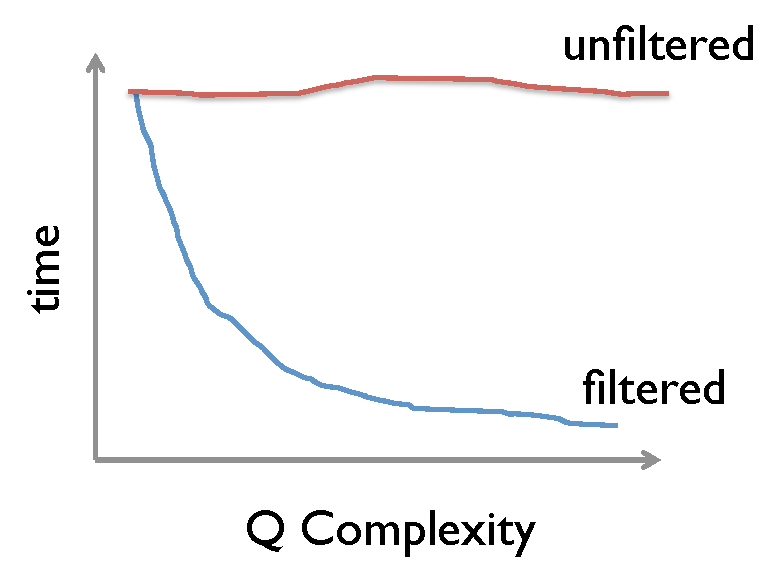
\includegraphics[width = 2in]{figures/complete_qfilter_complexity}
  \caption{Varying query complexity.}
  \label{f:complete_qfilter_complexity} 
  \end{figure}



  \subsection{Multi-Query}

  Using a previous experimental configuration, we varied the number of queries that are corrupted.  Figures~\ref{}
  show the quality and running times of the results for a query log of size 1000 and dbsize of 100k.  
  As we can see, the cost increases quadratically with each corrupted query and the accuracy of the proposed fixes increases marginally.  
  This is because XXX.

  We focus on two scenarios.  {\bf Try multiple corruptions that don't overlap (provenance-wise) with each other}.  This is the condition of multiple silo'd that
  corrupt their own logs.  Then {\bf Try multiple corrupted queries where one query modifies the updated state of the other}.  This shows that
  it is really hard and hopefully we get close?



  To better understand the algorithm, we plot the quality metrics after each fixed query and measure how quickly \sys converges to the final result. 
  This suggests that an incremental approach where the user can set a threshold to stop the algorithm may be effective.



  \subsection{Real Transactional Workload}

  We used the web application workload, and evaluated our alogirthms with artifically injected corruptions.
  We compared two types of corruptinos.  In figure~\ref{f:real_existing}, we randomly picked a single existing 
  query and corrupted its value.  If the query was an INSERT, we randomly pick a value and perturbed it.
  If the transaction was an UPDAET, we randomly varied the SET or WHERE clauses.   We re-ran this
  100 times and plot the average and standard deviation of the results.

}
